\documentclass[tikz,border=6pt]{standalone}
\usepackage[T1]{fontenc}
\usepackage{times}
\usepackage{amsmath,amssymb}
\usetikzlibrary{positioning,arrows.meta,calc,backgrounds}

% palette matching the project style
\definecolor{encC}{HTML}{5B7D9A}   % steel blue (encoder)
\definecolor{decC}{HTML}{B5805A}   % warm sienna (decoder)
\definecolor{s1C}{HTML}{5B7D9A}    % stage 1 - detection
\definecolor{s2C}{HTML}{5A8E72}    % stage 2 - categorization
\definecolor{xaiC}{HTML}{B5805A}   % stage 2.1 - explainability
\definecolor{s3C}{HTML}{7B6B8A}    % stage 3 - diagnosis
\definecolor{darkC}{HTML}{2D2D2D}
\definecolor{grayC}{HTML}{777777}
\definecolor{ioC}{HTML}{999999}

\begin{document}
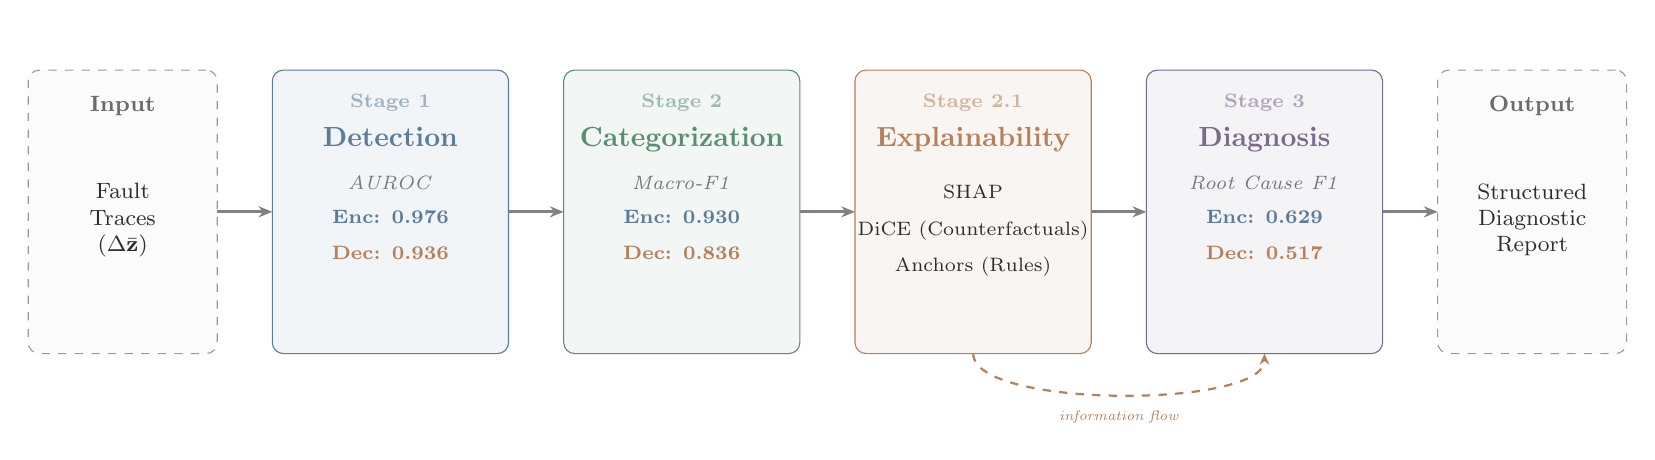
\begin{tikzpicture}[
  >=Stealth,
  every node/.style={font=\rmfamily, text=darkC},
  stagebox/.style 2 args={
    draw=#1, fill=#1!8, rounded corners=4pt,
    minimum width=3.0cm, minimum height=3.6cm,
    inner sep=0pt, outer sep=0pt,
  },
  iobox/.style={
    draw=ioC, dashed, fill=ioC!4, rounded corners=4pt,
    minimum width=2.4cm, minimum height=3.6cm,
    inner sep=0pt, outer sep=0pt,
  },
  mainflow/.style={-{Stealth[length=5pt,width=4pt]}, darkC!60, line width=1.0pt},
  evidflow/.style={-{Stealth[length=4pt,width=3.5pt]}, xaiC, line width=0.8pt, dashed},
]

% ── Input box ──
\node[iobox] (input) {};
\node[font=\rmfamily\small\bfseries, text=darkC!60] at ([yshift=12pt]input.north) {};
\node[font=\rmfamily\footnotesize\bfseries, text=darkC!70,
      anchor=north] at ([yshift=-6pt]input.north) {Input};
\node[font=\rmfamily\footnotesize, text=darkC, align=center]
      at ([yshift=-3pt]input.center) {Fault\\Traces\\($\Delta\bar{\mathbf{z}}$)};

% ── Stage 1: Detection ──
\node[stagebox={s1C}{}, right=0.7cm of input] (s1) {};
\node[font=\rmfamily\scriptsize\bfseries, text=s1C!60,
      anchor=north] at ([yshift=-5pt]s1.north) {Stage 1};
\node[font=\rmfamily\normalsize\bfseries, text=s1C,
      anchor=north] at ([yshift=-17pt]s1.north) {Detection};
\node[font=\rmfamily\scriptsize, text=grayC, anchor=north]
      at ([yshift=-35pt]s1.north) {\textit{AUROC}};
\node[font=\rmfamily\scriptsize\bfseries, text=encC, anchor=north]
      at ([yshift=-47pt]s1.north) {Enc: 0.976};
\node[font=\rmfamily\scriptsize\bfseries, text=decC, anchor=north]
      at ([yshift=-60pt]s1.north) {Dec: 0.936};

% ── Stage 2: Categorization ──
\node[stagebox={s2C}{}, right=0.7cm of s1] (s2) {};
\node[font=\rmfamily\scriptsize\bfseries, text=s2C!60,
      anchor=north] at ([yshift=-5pt]s2.north) {Stage 2};
\node[font=\rmfamily\normalsize\bfseries, text=s2C,
      anchor=north] at ([yshift=-17pt]s2.north) {Categorization};
\node[font=\rmfamily\scriptsize, text=grayC, anchor=north]
      at ([yshift=-35pt]s2.north) {\textit{Macro-F1}};
\node[font=\rmfamily\scriptsize\bfseries, text=encC, anchor=north]
      at ([yshift=-47pt]s2.north) {Enc: 0.930};
\node[font=\rmfamily\scriptsize\bfseries, text=decC, anchor=north]
      at ([yshift=-60pt]s2.north) {Dec: 0.836};

% ── Stage 2.1: Explainability ──
\node[stagebox={xaiC}{}, right=0.7cm of s2] (xai) {};
\node[font=\rmfamily\scriptsize\bfseries, text=xaiC!60,
      anchor=north] at ([yshift=-5pt]xai.north) {Stage 2.1};
\node[font=\rmfamily\normalsize\bfseries, text=xaiC,
      anchor=north] at ([yshift=-17pt]xai.north) {Explainability};
\node[font=\rmfamily\scriptsize, text=darkC, anchor=north]
      at ([yshift=-38pt]xai.north) {SHAP};
\node[font=\rmfamily\scriptsize, text=darkC, anchor=north]
      at ([yshift=-51pt]xai.north) {DiCE (Counterfactuals)};
\node[font=\rmfamily\scriptsize, text=darkC, anchor=north]
      at ([yshift=-64pt]xai.north) {Anchors (Rules)};

% ── Stage 3: Diagnosis ──
\node[stagebox={s3C}{}, right=0.7cm of xai] (s3) {};
\node[font=\rmfamily\scriptsize\bfseries, text=s3C!60,
      anchor=north] at ([yshift=-5pt]s3.north) {Stage 3};
\node[font=\rmfamily\normalsize\bfseries, text=s3C,
      anchor=north] at ([yshift=-17pt]s3.north) {Diagnosis};
\node[font=\rmfamily\scriptsize, text=grayC, anchor=north]
      at ([yshift=-35pt]s3.north) {\textit{Root Cause F1}};
\node[font=\rmfamily\scriptsize\bfseries, text=encC, anchor=north]
      at ([yshift=-47pt]s3.north) {Enc: 0.629};
\node[font=\rmfamily\scriptsize\bfseries, text=decC, anchor=north]
      at ([yshift=-60pt]s3.north) {Dec: 0.517};

% ── Output box ──
\node[iobox, right=0.7cm of s3] (output) {};
\node[font=\rmfamily\footnotesize\bfseries, text=darkC!70,
      anchor=north] at ([yshift=-6pt]output.north) {Output};
\node[font=\rmfamily\footnotesize, text=darkC, align=center]
      at ([yshift=-3pt]output.center) {Structured\\Diagnostic\\Report};

% ── Main flow arrows ──
\draw[mainflow] (input.east) -- (s1.west);
\draw[mainflow] (s1.east) -- (s2.west);
\draw[mainflow] (s2.east) -- (xai.west);
\draw[mainflow] (xai.east) -- (s3.west);
\draw[mainflow] (s3.east) -- (output.west);

% ── Information flow (dashed, curving below) ──
\draw[evidflow]
    (xai.south) .. controls ++(0,-0.7) and ++(0,-0.7) .. (s3.south)
    node[pos=0.5, below=2pt,
         font=\rmfamily\tiny\itshape, text=xaiC] {information flow};

\end{tikzpicture}
\end{document}
